\begin{exercisePage}
	\setcounter{taskcount}{24}
	\begin{task}
		Es seien $g\in C^2_0(\mathbb R)$ und $h \in C_0^1(\mathbb{R})$ Funktionen mit kompaktem Träger, und es sei $u \in C^2(\mathbb{R}\times [0,\infty))$ eine Lösung der homogenen Wellengleichung
		\begin{equation*}
		\begin{cases}
		u_{tt}-u_{xx} = 0  &\text{ auf } \mathbb{R} \times (0,\infty),
		\\
		u = g \mbox{ , } u_t = h &\text{ auf } \mathbb{R} \times \{0\}.
		\end{cases}
		\end{equation*}
		Die \enquote{kinetische Energie} $k$ und die \enquote{potentielle Energie} $p$ seien definiert durch
		\begin{equation*}
			k(t) \defeq \frac12 \int_{-\infty}^\infty u_t^2(x,t) \dx
			\quad \und \quad 
			p(t) \defeq \frac12 \int_{-\infty}^\infty u_x^2(x,t)\dx\quad (t>0)
		\end{equation*}
		Zeigen Sie:
		\begin{enumerate}
			\item $k + p$ ist konstant.
			\item $k(t) = p(t)$ für alle genügend großen $t$.
		\end{enumerate}
	\end{task}

	\begin{enumerate}[label=(zu \alph*), leftmargin=*]
		\item Wir betrachten die Formel von d'Alembert 
		\begin{equation*}
			u(x,t) = \frac{1}{2} \brackets{g(x+t) + g(x-t)} + \frac{1}{2} \int_{x-t}^{x+t} h(y) \dy
		\end{equation*}
		Das Integral können wir mittels $y=x+zt$ und $\diff{y} = t \diff{z}$ transformieren zu $t * \int_{-1}^1 h(x+zt) \dz$. Damit können wir problemlos nach $x$ und $t$ ableiten, wobei aufgrund der kompakten Träger die Reihenfolge von Integration und Differentiation vertauschbar ist. Es gilt also:
		\begin{align*}
			u_x(x,t) 
			&= \frac{1}{2} \brackets{g'(x+t) + g'(x-t) + t \int_{-1}^1 h'(x+zt) \dz} \\
			&= \frac{1}{2} \brackets{g'(x+t) + g'(x-t) + h(x+t) - h(x-t} \\
			u_{xx}(x,t) 
			&= \frac{1}{2} \brackets{g''(x+t) + g''(x-t) + h'(x+t)  - h'(x-t)} \\
			u_{xt}(x,t) 
			&= \frac{1}{2}  \brackets{g''(x+t) - g''(x-t) + h'(x+t) + h'(x-t)} \\
			u_t(x,t)
			&= \frac{1}{2} \brackets{g'(x+t) - g'(x-t) + \int_{-1}^1 h(x+zt) \dz + t \int_{-1}^1 h'(x+zt) * z \dz} \\
			&= \frac{1}{2} \brackets{g'(x+t) - g'(x-t) + h(x+t) + h(x-t)}
		\end{align*}
		Wir wollen nun zeigen, dass
		\begin{equation*}
			(k+p)'(t) = \frac{1}{2} \ableitung{t} \int_{-\infty}^\infty u_t^2(x,t) + u_x^2(x,t) \dx 
			= \int_{-\infty}^\infty  u_t(x,t) \underbrace{u_{tt}(x,t)}_{= u_{xx}(x,t)} + u_x(x,t) u_{xt}(x,t) \dx
		\end{equation*}
		Durch Einsetzen und Ausmultiplizieren erhalten wir einen fürchterlichen Term:
		\begin{align*}
			&\tfrac{1}{2} u_t(x,t) u_{xx}(x,t) + u_x(x,t) u_{xt}(x,t) \\
			= \enskip &g'(x+t)g''(x+t) + g'(x+t)h'(x+t) - g'(x-t)g''(x-t) + g'(x-t)h'(x-t) + \\ 
			&h(x+t)g''(x+t) + h(x+t)h'(x+t) + h(x-t) g''(x-t) - h(x-t) h'(x-t)
		\end{align*}
		Nun sind in jedem Summanden die inneren Ableitungen nach $t$ gleich, das heißt die Vorzeichen spielen bei der Integration über $x$ keine Rolle und wir erhalten
		\begin{equation*}
			(k+p)'(t) = \int_{-\infty}^\infty 4 * \brackets{ g'(z) h'(z) + g''(z) h(z) } \dz
		\end{equation*}
		sowie mit partieller Integration für den zweiten Summanden
		\begin{equation*}
			\int_{-\infty}^\infty g''(z) h(z) \dz 
			= \sqbrackets{g'(z) h(z)}_{-\infty}^\infty - \int_{-\infty}^\infty g'(z) h'(z) \dz 
			= - \int_{-\infty}^\infty g'(z) h'(z) \dz
		\end{equation*}
		Damit ist nun schlussendlich 
		\begin{equation*}
			\begin{aligned}
				(k+p)'(t) 
				&= 4 * \int_{-\infty}^\infty g'(z) h'(z) \dz +  4 * \int_{-\infty}^\infty g''(z) h(z) \dz \\
				&= 4 * \int_{-\infty}^\infty g'(z) h'(z) \dz - 4 * \int_{-\infty}^\infty g'(z) h'(z) \dz = 0
			\end{aligned}
		\end{equation*}
		und folglich also $k+p$ konstant für alle $t > 0$.
		
		\item Betrachten wir nun $k-p$. Der ausmultiplizierte Integrant ergibt sich als
		\begin{equation*}
			u_x^2(x,t) - u_t^2(x,t) = g'(x+t) g'(x-t) - g'(x+t) h(x-t) + g'(x-t) h(x+t) - h(x+t) h(x-t) 
		\end{equation*}
		Die Funktionen $g$ und $h$ leben auf kompakten Trägern, d.h. es existieren Radien $R_g, R_h > 0$, sodass $\supp(g) \subseteq B_{R_g}(0)$, $\supp(h) \subseteq B_{R_h}(0)$ und auch $\supp(g') \subseteq B_{R_g}(0)$. Ist $t$ nun hinreichend groß, d.h. $t > R \defeq \menge{R_g, R_h}$, dann ist $x+t \notin B_R(0)$ oder $x-t \notin B_R(0)$. Somit wird stets einer der beiden Faktoren in obigen Summanden außerhalb des Trägers liegen und somit gleich Null sein. Das heißt also, dass $u_x^2(x,t) - u_t^2(x,t) = 0$  für alle $t > R$ und $x \in R$ bzw. $p(t) - k(t) = 0 \equiv p(t) = k(t)$ für hinreichend große $t$.
	\end{enumerate}
	
	
	
	\begin{task}
		Es seien $g,h \in C_0^\infty(\mathbb{R}^3)$ gegeben und es sei $u \in C^2(\mathbb{R}^3\times [0,\infty))$ eine Lösung der homogenen Wellengleichung
		\begin{equation*}
		\begin{cases}
		u_{tt}-\Delta u = 0  &\text{ auf } \mathbb{R}^3 \times (0,\infty),
		\\
		u = g \mbox{ , } u_t = h &\text{ auf } \mathbb{R}^3 \times \{0\}.
		\end{cases}
		\end{equation*}
		Zeigen Sie:
		\begin{equation*}
			\exists C > 0 ~\forall x \in \mathbb R^3, t \in (0,\infty): \abs{u(x,t)} \leq \frac{C}{t}
		\end{equation*}
		Schätzen Sie dazu $u(x,t)$ auf geeigneten Teilbereichen von $\mathbb{R}^3\times [0,\infty)$ ab.
	\end{task}

	Mit der Kirchhoff'schen Formel erhalten wir als Darstellung der Lösung
	\begin{equation*}
		u(x,t) = \frac{1}{3 t^2 \alpha(3)} \int_{\rand B_t(0)} t h(x+z) + g(x+z) + Dg(x+z) * z \diffskip{O(z)}
	\end{equation*}
	Schreibe von nun an $\alpha \defeq \alpha(3)$. Gemäß Voraussetzung leben $g$ und $h$ auf kompakten Trägern, d.h. es existieren Radien $R_g, R_h >0$, sodass $\supp(g) \subseteq B_{R_g}(0)$ und $\supp(h) \subseteq B_{R_h}(0)$ sowie insbesondere auch $\supp(Dg) \subseteq B_{R_g}(0)$. Auf diesen kompakten Trägern nehmen die stetigen Funktionen auch ein Maximum an, d.h. $g(x) \le g_{\max} \defeq \max_{x \in \R^3}\abs{g(x)}$, $h(x) \le h_{\max} \defeq \max_{x \in \R^3}\abs{h(x)}$, $Dg(x) \le g'_{\max} \defeq \max_{x \in \R^3}\abs{Dg(x)}$ für alle $x \in \R^3$. 
	Dann gilt mit $R \defeq \max\menge{R_g, R_h}$ für $t \le R$
	\begin{align*}
			\abs{u(x,t)} 
			&\le \frac{1}{3 t^2 \alpha} \int_{\rand B_t(0)} \abs{t} * \abs{h(x + z)} + \abs{g(x + z)} + \abs{Dg(x+z)} * \abs{z} \diffskip{O(z)} \\
			&\le \frac{1}{3 t \alpha} \int_{\rand B_R(0)} h_{\max} \diffskip{O(z)}
			+ \frac{1}{3 t^2 \alpha} \int_{\rand B_R(0)} g_{\max} \diffskip{O(z)}
			+ \frac{1}{3 t \alpha} \int_{\rand B_R(0)} g'_{\max} \diffskip{O(z)}\\
			&= \frac{R^2 h_{\max}}{t} + \frac{R^2 h_{\max}}{t^2} + \frac{R^2 g'_{\max}}{t} \tag{$\abs{\rand B_R(0)} = R^2 * 3\alpha$}
	\end{align*}
	Für hinreichend große $t$ ist $\frac{1}{t} \approx \frac{1}{t^2}$, d.h. mit $C_1 \defeq R^2 \brackets{h_{\max} + g_{\max} + g'_{\max}} > 0$ gilt die Abschätzung $\abs{u(x,t)} \le \frac{C_1}{t}$. Für kleine $t$ in einer Umgebung der Null ist $u(x,t) \overset{t \to 0}{\longrightarrow} \abs{g(x)} \le g_{\max}$ beschränkt, d.h. ex existiert ein $C_1'> 0$, sodass $\abs{u(x,t)} \le \frac{C_1'}{t}$. 
	
	\begin{wrapfigure}{r}{6cm}
		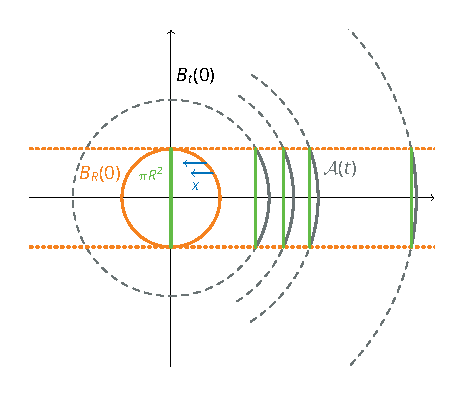
\includegraphics[width=6cm]{pde-uebungen-9-abb.pdf}
	\end{wrapfigure}
	Sein nun $t > R$. In diesem Fall muss $x+z$ nicht mehr unbedingt in den jeweiligen Trägern von $g$ oder $h$ liegen. Dies ist jedoch der Fall, wenn $\abs{x+z} < R$. Wählen wir nun ein $z \in \rand B_R(0)$, d.h. auf dem Rand der $R$-Kugel, die kleiner ist als die $t$-Kugel. Für ein fixiertes $x$ kann die Bedingung $\abs{x+z} < R$ höchstens für eine Hemisphäre gelten (für die jeweils andere Hemisphäre \enquote{zeigt $x$ aus der Kugel}). Der Flächeninhalt einer solchen Sphäre ist $\mathcal{A}(t) = \pi R^2 + \omega(t)$, wobei $\omega(t)$ den Flächenzuwachs durch die Wölbung der $t$-Kugel beschreibt. Je größer $t$ wird, desto geringer wird die Wölbung, da der \enquote{Ausschnitt} der gleiche bleibt, d.h. $\omega$ fällt monoton und für $t \to \infty$ gilt $\omega(t) \to 0$, d.h. $\mathcal{A}(t) \to \pi R^2$. Somit ist $\mathcal{A}$ beschränkt durch $\pi R^2 \le \mathcal{A}(t) \le \pi R^2 + \omega(R)$ für alle $t > R$. Somit ist
	\begin{align*}
		\abs{u(x,t)} 
		&\le \frac{1}{3 t^2 \alpha} \int_{\rand B_t(0)} \abs{t h(x+z)} + \abs{g(x+z)} + \abs{Dg(x+z)} * \abs{z} \diffskip{O(z)} \\
		&\le \mathcal{A}(t) * \brackets{\frac{h_{\max}}{3t\alpha} + \frac{g_{\max}}{3t^2\alpha} + \frac{g'_{\max}}{3t\alpha}} \\
		&= \underbrace{\mathcal{A}(t) \frac{h_{\max} + g_{\max} + g'_{\max}}{3\alpha}}_{\defqe C_2} * \frac{1}{t} = \frac{C_2}{t}
	\end{align*}
	Definiere abschließend $C \defeq \max\menge{C_1, C_1', C_2}$, dann ist $\abs{u(x,t)} \le \frac{C}{t}$ für alle $(x,t) \in \R^3 \times (0, \infty)$.
\end{exercisePage}